\newpage
\chapter*{Testbed Build and Verification}
\addcontentsline{toc}{chapter}{Testbed Build and Verification}
The NASA Radio Jove dual dipole antenna design (Figure: \ref{fig:dual_dipole_antenna_array}) was chosen over the other designs for a number of reasons, namely:

\begin{itemize}
	\item Simplicity of the architecture and consequently also construction
	\item Low cost of building materials
	\item Reasonably effective performance (5-9 dB gain depending on configuration)
	\item Easy to operate and maintain
	\item Suitable for a permanent installation
	\item Large body of technical documentation supporting the operation
\end{itemize}


\section*{Special Resources Required}
\addcontentsline{toc}{section}{Special Resources Required}
% The research work may require access to specialised equipment, software, journals and so on.

The following resources have been identified as being required in order to perform the research and are listed as follows:

\begin{description}
  \item[GnuRadio] \hfill \\
  The GnuRadio software is an open-source software development tool kit that allows access to signal processing techniques in order to implement software radio solutions.
  \item[HackRF] \hfill \\
  The HackRF \gls{SDR} transceiver system is the software defined radio transceiver chosen for the prototype system.
  \item[PL259 / SO239] \hfill \\
  Cable adapters which connect coax cables together with the dipole center.
  \item[Radio Jove Software] \hfill \\
  The Radio Jove software is extremely useful for observers wishing to capture \gls{DAM} emissions from Jupiter. It contains a large number of features such as emission prediction observation charts, and information regarding Jupiter's location in the sky from any specified point on the Earth's surface.
  \item[RG59 Coax] \hfill \\
  RG59 coax cable is required to link the dipole antennas back to the \gls{SDR} transceiver.
  \item[Spectrum Analyser] \hfill \\
  A spectrum analyser will be required in order to perform a site survey to determine if a location is suitable for collecting \gls{DAM} emissions.
\end{description}


\section*{Antenna Build}
\addcontentsline{toc}{section}{Antenna Build}

\newglossaryentry{SWR}
{
  name={SWR},
  description={Standing Wave Ratio is the ratio of the maximum peak voltage
  	anywhere on a line to the minimum value anywhere along a line},
  sort=SWR
}

In order to satisfy the main requirement of capturing \gls{DAM} signals at 20.1MHz construction of an antenna was needed. The equation shown in Figure: \ref{fig:wavelength_equation_wire_antenna} was used to calculate a starting estimate of the length of antenna wire required to construct this antenna. Many factors can affect the ability of an antenna to receive data at a particular frequency \citep{arrl-00}, such as the following:

\begin{itemize}
	\item quality of the wire conductor or thickness of the wire
	\item height that the antenna is mounted above the ground
	\item capacitive end effects
	\item closeness to radio conductors
\end{itemize}

One simple method of partly improving antenna performance is by controlling the length of the antenna wire while measuring the Standing Wave Ratio (\gls{SWR}) value, which is the ratio of the maximum peak voltage anywhere on a line to the minimum value at any point along the same line. The use of a \gls{SWR} analyser becomes invaluable in this process.

%
\begin{figure}[here]
\centering
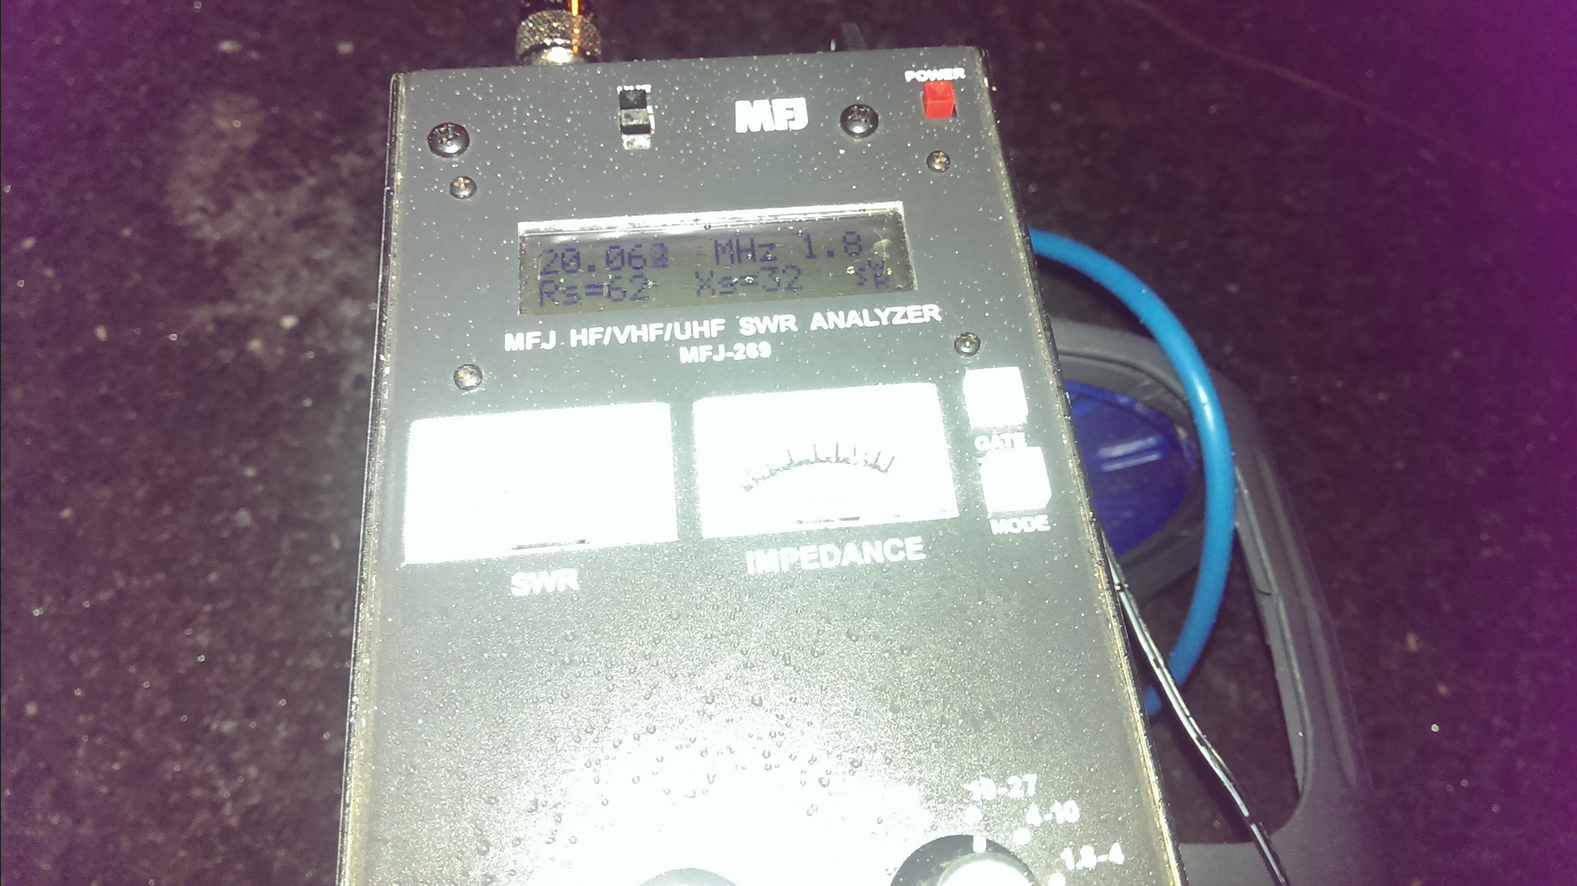
\includegraphics[width=8cm]{images/34}
\caption{Measuring the SWR of the antenna with an SWR Analyser}
\label{fig:swr_analyser_measuring_antenna}
\end{figure}
%

The initial length of antenna wire was cut to match the length produced by the equation in Figure: \ref{fig:wavelength_equation_wire_antenna} and was then cut in half before each end was connected to a dipole centre. The antenna was placed on the ground before being connected to the \gls{SWR} analyser. The \gls{SWR} value for the antenna was measured, and it was discovered the antenna was suitable for capturing of signals at 18 MHz. The antenna was then shortened by a small identical amount on each side and the \gls{SWR} values were again measured until the antenna registered as being most suitable for operation at 20.1MHz as seen in Figure:  \ref{fig:swr_analyser_measuring_antenna}. 

The \gls{SWR} equations shown in Figure: \ref{fig:swr_equation} $|\rho|$ is the reflection coefficient, P$_{f}$ is the power in the forward wave entering the antenna while P$_{r}$ is the power of the reflected wave in the antenna \citep{arrl-00}.

%
\begin{figure}[here]
  \centering
  \begin{equation}
  	SWR = \frac{1 + |\rho|}{1 - |\rho|} 
  \end{equation}
  \begin{equation}
  	|\rho| = \frac{SWR - 1}{SWR + 1} 
  \end{equation}
  \begin{equation}
  	|\rho| = \sqrt{\frac{P_r}{P_f}}
  \end{equation}
  \caption{Standing Wave Ratio Equations}
  \label{fig:swr_equation}
\end{figure}
%

%
\begin{figure}[here]
  \centering
  \begin{equation}
  	|\rho| = \frac{1.2 - 1}{1.2 + 1} 
  \end{equation}
  \begin{equation}
  	|\rho| = 0.09090909090909088
  \end{equation}
  \begin{equation}
  	0.09090909090909088 = \sqrt{\frac{P_r}{100}}
  \end{equation}
  \begin{equation}
  	0.09090909090909088^2 = \frac{P_r}{100}
  \end{equation}
  \begin{equation}
  	P_r = 0.826446280991735
  \end{equation}
  \caption{Calculating P$_{r}$ for the antenna}
  \label{fig:swr_equation_pr}
\end{figure}
%

The value of \gls{SWR} for the antenna should be ideally as close as possible to 1, this ensures all the signal energy collected by the antenna is transferred to the load successfully. However in practice this is never the case as all antennas have varying amounts of loss. The antenna once mounted had a measured \gls{SWR} value of 1.2 which equates to a P$_{r}$ value as shown in Figure: \ref{fig:swr_equation_pr} of 0.826446280991735 which is a loss of 17.35\% or about 1dB which is considered reasonable \citep{arrl-00}.

\newpage
Table: \ref{tab:sdrt_build_cost} gives a breakdown of the costs associated with the antenna build to date. While Table: \ref{tab:radio_jove_kit_cost} gives the breakdown of the official NASA Radio Jove kit for comparison.

%
\begin{table}
  \centering
  \begin{tabular}{p{8cm} l}
    \toprule
    Item Name & Cost (\euro) \\ \midrule
    100m Copper Wire & 20.00  \\
    100m Coax RG59 & 25.00  \\
    2 $\times$ Dipole Centers & 20.00 \\
    8 $\times$ PL259 & 18.00 \\
    2 $\times$ SO239 & 4.00 \\
    SMA-SO239 Adapter & 4.50 \\
    2 $\times$ SO239-SO239 Adapter & 4.50 \\
    T Adapter & 3.00 \\
    Patch Lead & 5.00 \\
    2 $\times$ 4m 5cm Pipe & 15.00 \\
    2 $\times$ 4m 4cm Pipe & 15.00 \\
    HackRF Transceiver & 315.00 \\
    RTL DAB Receiver & 25.00 \\
    MCX-SO239 Adapter & 6.50 \\
    \bottomrule
    \\
    Total & 480.00
  \end{tabular}
  \caption{SDRT Build Cost}
  \label{tab:sdrt_build_cost}
\end{table}
%

%
\begin{table}
	\centering
	\begin{tabular}{p{8cm} l}
		\toprule
		Item Name & Cost (\euro) \\ \midrule
		RF 2080 Calibrator/Filter & 100.00  \\
		Receiver & 295.00  \\
		Antenna Kit & 65.00 \\
		International shipping & 60.00 \\
		\bottomrule
		\\
		Total & 520.00
	\end{tabular}
	\caption{SDRT Build Cost \citep{nasa14}}
	\label{tab:radio_jove_kit_cost}
\end{table}
%

\newpage
\section*{Listening Site Suitability}
\addcontentsline{toc}{section}{Listening Site Suitability}
A convenient location for the antenna deployment was selected and the antenna was deployed. It was necessary to determine if this site was in fact a suitable location to host a radio telescope antenna. In order measure the ambient noise at the site, a Tektronics SA2600 spectrum analyser was connected to the antenna and left for 2 hours at midday to gather data. The spectrum is likely to be full of radio interference from human and natural sources at this time. The results can be seen in Figure: \ref{fig:site_survey_spec_analyser}. The ambient \gls{RF} noise at the site was quite high, ranging between -80dB and -70dB on average. 

\newglossaryentry{preamp}
{
  name={preamp},
  description={pre-amplifier - is an electronic amplifier that prepares a small electrical signal for further amplification or processing},
  sort=preamp
}

Similar readings were taken using the HackRF while attached to the antenna as show in Figure: \ref{fig:site_survey_hackrf}. The measurements recorded with the HackRF were performed using the \textit{gqrx} \gls{SDR} software while all amplification settings inside \textit{gqrx} were set at 0, in order to get an accurate reading on the raw signal being collected by the antenna. The values were on average -20dB quieter than those recorded by the SA2600 spectrum analyser, this points towards an inherent deafness flaw in the HackRF design itself, and possibly the requirement of a pre-amplifier (\gls{preamp}) in order to boost the gain on the input signal. 

\newglossaryentry{RF}
{
  name={RF},
  description={Radio Frequency is a rate of oscillation which corresponds to the frequency of a radio wave},
  sort=RF
}

%
\begin{figure}	
	\centering
	\begin{subfigure}[t]{5cm}
		\centering
		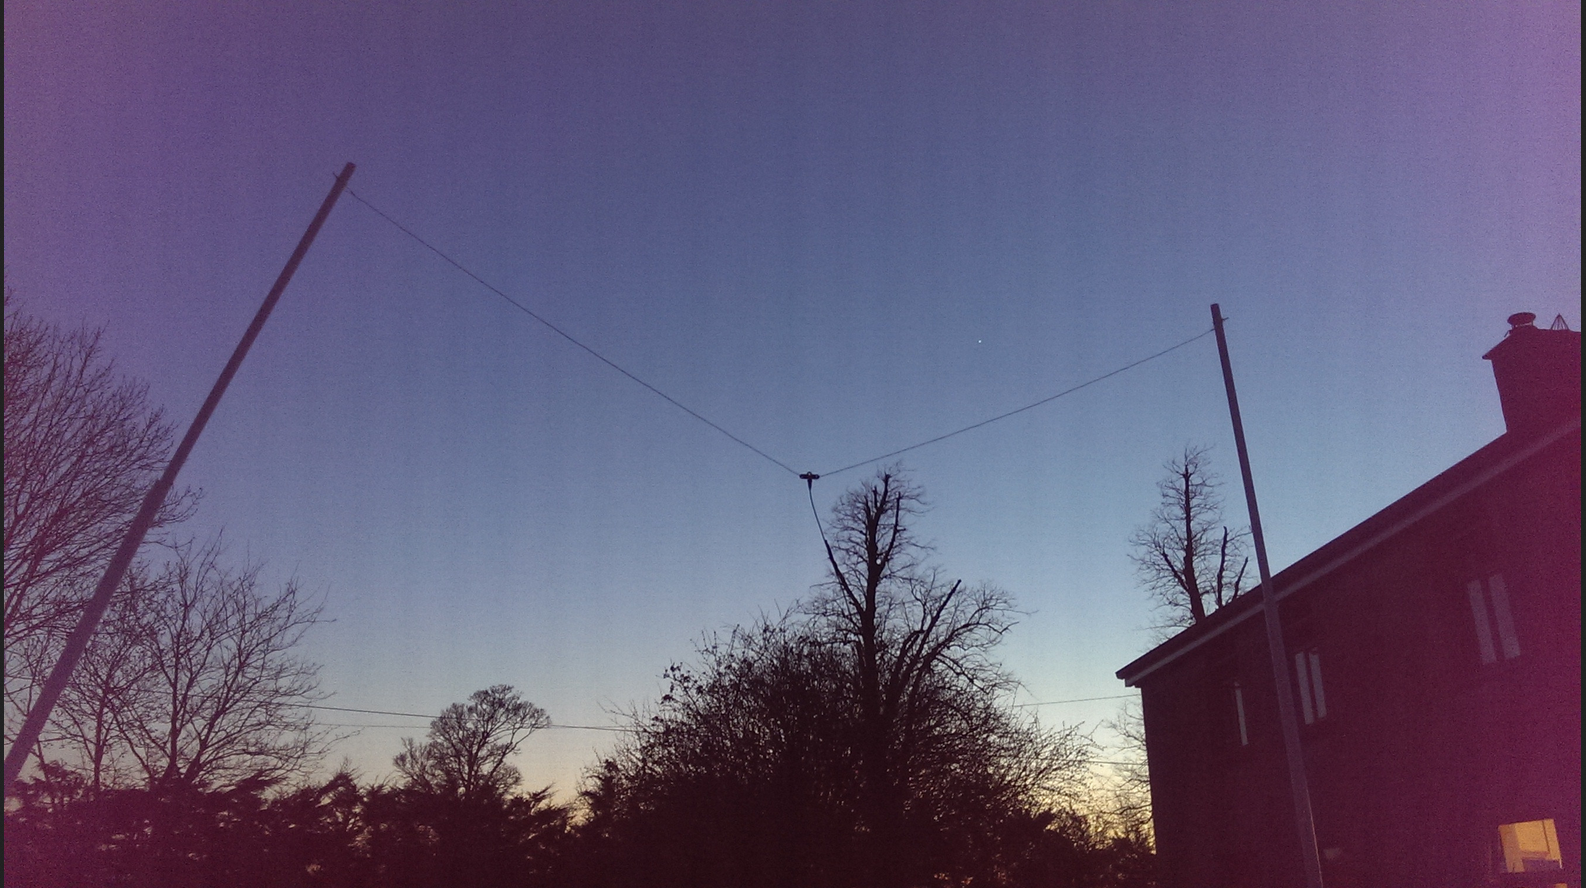
\includegraphics[width=5cm]{images/32}
		\caption{Dual Dipole Antenna Deployment}
		\label{fig:dual_dipole_deployed}
	\end{subfigure}
	\quad
	\begin{subfigure}[t]{5cm}
		\centering
		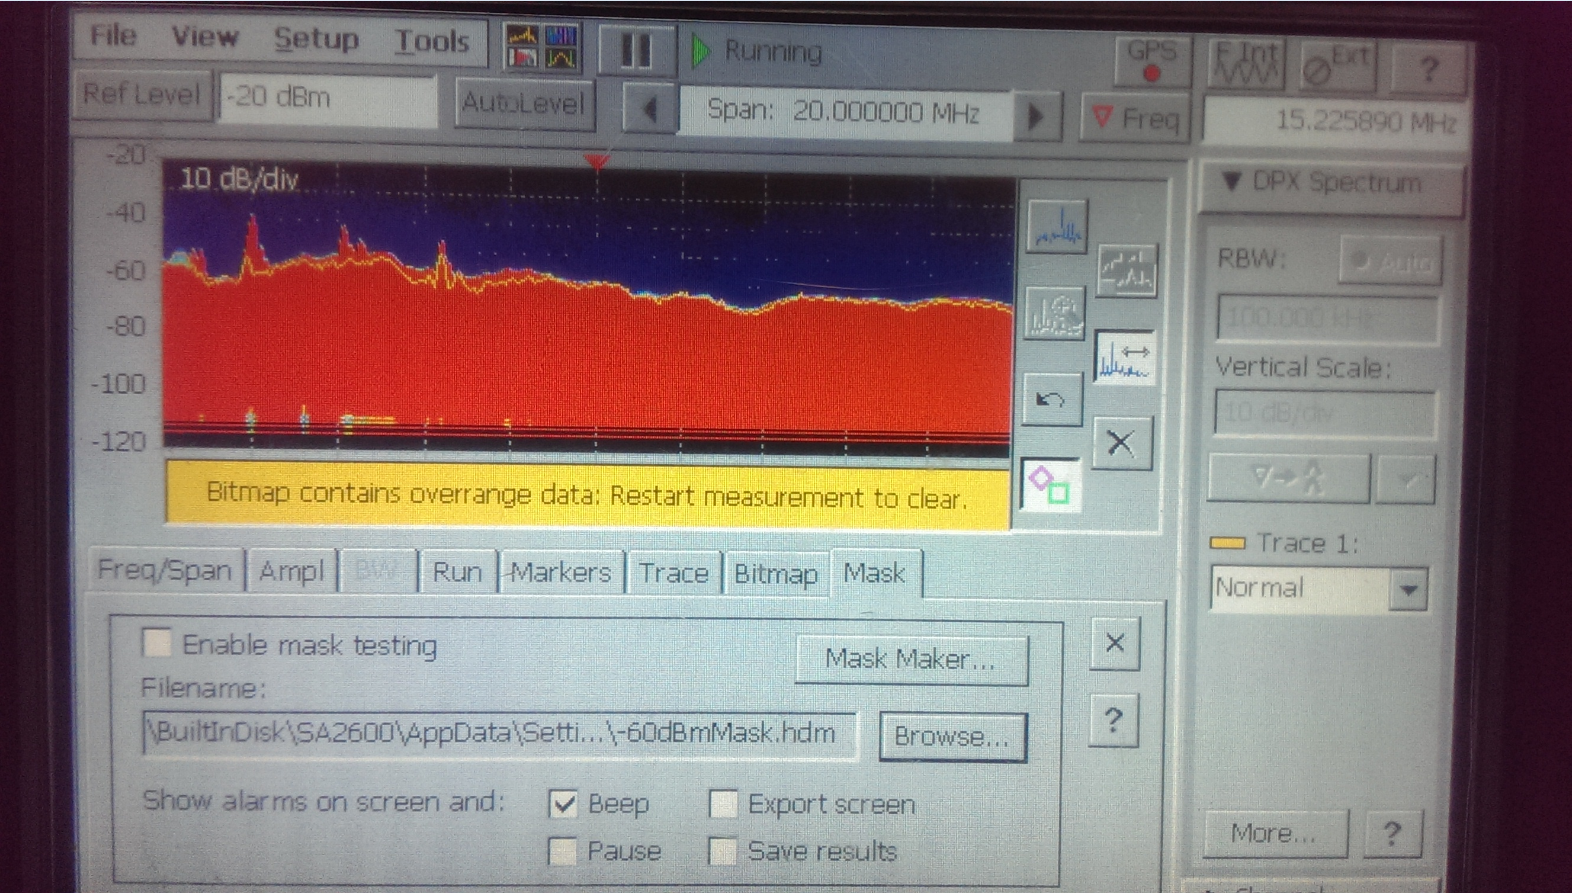
\includegraphics[width=5cm]{images/26}
		\caption{Site Survey performed using a Tektronics SA2600 Spectrum Analyser}
		\label{fig:site_survey_spec_analyser}
	\end{subfigure}
	\quad
	\begin{subfigure}[t]{5cm}
		\centering
		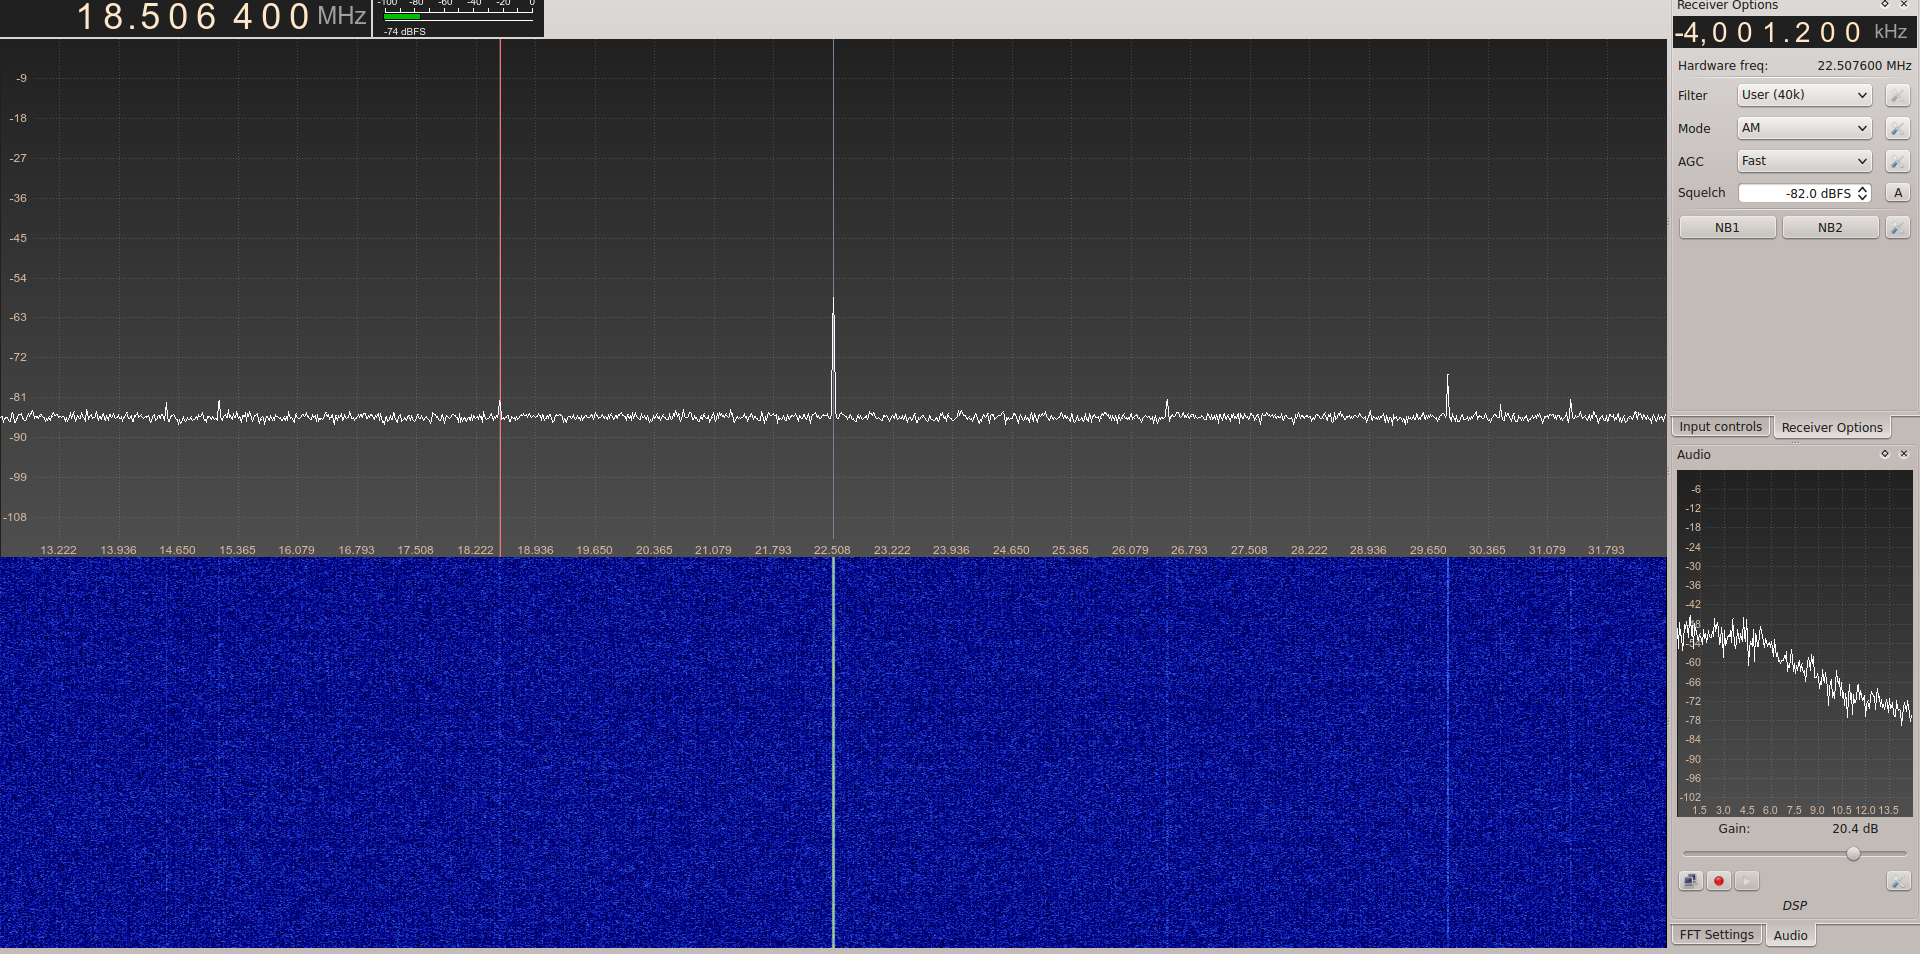
\includegraphics[width=5cm]{images/31}
		\caption{Site Survey performed using HackRF One}
		\label{fig:site_survey_hackrf}
	\end{subfigure}
	\quad
	\begin{subfigure}[t]{5cm}
		\centering
		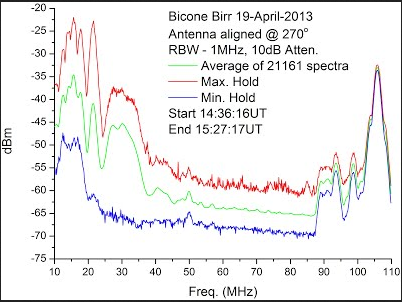
\includegraphics[width=5cm]{images/35}
		\caption{LOFAR Site Suitability Survey performed at Birr Castle \citep{craf-13}}
		\label{fig:site_survey_lofar}
	\end{subfigure}
	\caption{Site Survey}
	\label{fig:site_survey}
\end{figure}
%

\newglossaryentry{LOFAR}
{
  name={LOFAR},
  description={Low Frequency Array - radio interferometer constructed in the north of the Netherlands and across europe https://www.astron.nl/lofar-telescope/lofar-telescope},
  sort=LOFAR
}

In May 2013, the Solar Physics Group from Trinity College Dublin, performed a site survey at Birr Castle to ascertain the suitability of the site for an installation of the Low Frequency Array (\gls{LOFAR}) telescope \citep{craf-13}. The study was focused on a wide range of frequencies between 10 and 400MHz, a portion of which can be seen in Figure: \ref{fig:site_survey_lofar}. The report concluded that the location at Birr Castle was a relatively quiet location as compared against a site at Bornim, Germany and another at Bleien, Switzerland. 

From the results of this survey, it can be seen that the average background noise levels were about -55dB near 20MHz which is similar to those recorded 80km away at the Kilkenny site. Table: \ref{tab:site_survey} details the results collected at the Kilkenny site and includes those performed by the Solar Physics Group at Birr Castle for comparison. Results indicate the Kilkenny site appears to be a reasonable location at which to host the radio telescope.


%
\begin{table}
  \centering
  \begin{tabular}{p{2cm} l r}
    \toprule
    Site & Equipment & Average Noise at 20.1MHz \\ \midrule
    Kilkenny & Tektronix SA2600 20.1MHz Dipole & -65dB  \\
    Kilkenny & HackRF One 20.1MHz Dipole & -65dB \\
    Birr & LOFAR Array 10-100MHz Schwarzbeck Bicone & -55dB \\
    \bottomrule
  \end{tabular}
  \caption{Average Noise Measurements at Kilkenny Listening Site compared to Birr Listening Site \citep{craf-13}}
  \label{tab:site_survey}
\end{table}
%

\newglossaryentry{RSGB}
{
  name={RSGB},
  description={RSGB - The Radio Society of Great Britain http://rsgb.org/},
  sort=RSGB
}

\newglossaryentry{MW}
{
  name={MW},
  description={MW - Medium Wave frequencies usually in the wavelengths 300 kHz - 3 MHz},
  sort=RSGB
}


\section*{Verification of the Radio Receiver}
\addcontentsline{toc}{section}{Verification of the Radio Receiver}
An opportunity to validate the HackRF transceiver arose with the announcement of a public Medium Wave (\gls{MW}) experiment by \cite{RSGB-15-b} of the Radio Society of Great Britain (\gls{RSGB}). The \gls{RSGB} Propagation Studies Committee intended to perform an experiment during the partial solar eclipse on 20th March 2015. As can be seen in Figure: \ref{fig:solar_eclipse_scale}, the UK and Ireland would witness more than 90\% totality during the eclipse. This was an opportunity to perform simple experiments to demonstrate the Sun's effect on Earth's ionosphere, and how this ionisation affects the propagation of radio signals.

According to \cite{nichols-15-a}, \gls{MW} radio stations which are located more than 500 km away are unlikely to be propagated during daylight hours due to their signals being absorbed by the D layer as shown in Figure: \ref{fig:atmosphere_ionisation_effects_mw}. However this D layer does not exist during night time hours, as a result these radio signals are free to reflect from the E and F layers. \cite{RSGB-15-b} states that this is also true during a solar eclipse with a high totality percentage as would occur on the 20th March 2015.

%
\begin{figure}[!htb]
	\centering
	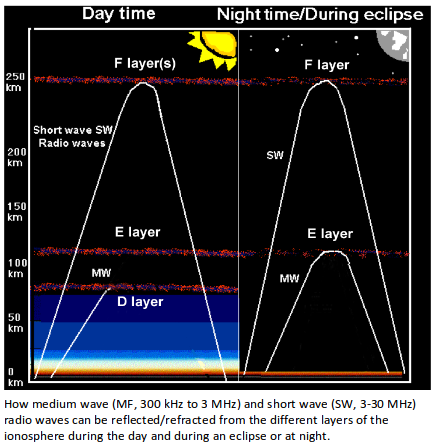
\includegraphics[width=8cm]{images/53}
	\caption{Comparing propagation of \gls{MW} radio signals during day and during night/solar eclipse \citep{RSGB-15-b}}
	\label{fig:atmosphere_ionisation_effects_mw}
\end{figure}
%

\cite{RSGB-15-b} provided some a number of radio stations which transmit signals in the \gls{MW} range at various locations in the United Kingdom, Europe and also a number in Iceland. The experiment called for choosing a station which is transmitting in the \gls{MW} range and is capable of being heard at the listeners location during the night time. This station should not be capable of being heard during the day time, the experiment called for a station which is further away than 500 km. The chosen radio station should then be tuned in to coincide with the beginning of the solar eclipse. The station receive power should be plotted against time. It was expected that the signal strength of the radio station should rise to a maximum which coincided with the solar eclipse maximum.

It was immediately apparent that the RadioJove antenna design would not be suitable for this experiment, and a suitable alternative was examined. During the initial research into potential designs a paper by \cite{litva-76} mentioned the use of a Beverage antenna for use in highly directional receivers such as early transatlantic radio communication experiments. Due to the simple nature of the Beverage antenna design, this was considered for use in this experiment.

\newpage
\subsection*{Methodology}
The following methodology was followed during this experiment:

\begin{enumerate}
	\item The dipole antenna built for use in the main part of the dissertation was not best suited for picking up signals in the \gls{MW} range so an alternative design was chosen. 
	\item A Beverage antenna was picked as it was easily aimed and had a simple design. The antenna very simply consisted of a copper wire 80 m long attached to a long wire antenna terminator which had an SO239 connector \citep{litva-76}.
	\item The listening site was longest in the East-West axis, and having the receiver positioned at the far west end of the site was most convenient. For this reason a radio station situation in an Easterly direction was picked.
	\item The antenna was aimed in the general direction of the radio station chosen, and simply placed on the ground.
	\item HackRF was tuned to the chosen radio station.
	\item 2 MHz bandwidth of the spectrum was recorded during the entire length of the solar eclipse, the signal strength of the radio station can be plotted against time at a later date using this recorded data.
	\item The \gls{SDR} receiver should have the automatic gain control switch off in order to get accurate power results. 
\end{enumerate}


The chosen radio station was \textit{Radio China International} (1.440 MHz) which was a powerful signal during the night time despite it being transmitted from Marnach in Luxembourg which is 950 km away from the listening site. Once the solar eclipse began, the HackRF \gls{SDR} receiver was tuned to 1.440 MHz with a bandwidth of 2MHz and \gls{IQ} samples were recorded. As the eclipse neared 20\% totality, the radio station began to emerge from the background noise at -55 dB. The signal rose steadily until the eclipse maximum point which was -28 dB, and then averaged at a level of -45dB as the totality value dropped. At 20\% of eclipse totality, the station faded once more before disappearing into to the background noise level at -55dB. The results were plotted in Figure: \ref{fig:signal_power_v_time_radio_propagation} and were submitted to \citet{RSGB-15-b} for inclusion in the overall experiment.

A number of issues with the HackRF \gls{SDR} transceiver were discovered during this experiment. The technical specifications show the operating range of the HackRF to be 10 MHz - 6 GHz \citep{ossmann-15-d}. In practice it possible to tune to frequencies below 4 MHz, even as low as 500kHz with a few caveats.

Reliable tuning proved a problem below 10MHz, when the HackRF was was power cycled, tuning to the same frequency in software would see the station vanish. It took trial and error find it it once more by scanning lower and higher until the station was reaquired. This is due to the internal signal oscillator being affected by many external variables such as temperature. To be certain of the exact frequency being monitored, an external clock source must be used to provide a signal reference to the system. 

The HackRF also appears to be quite deaf without maxing the IF and \gls{RF} amplifiers. While this could be solved by adding a \gls{preamp} at the antenna, such a step would also increase the level of background noise which might defeat the purpose.


%
\begin{figure}	
	\centering
	\begin{subfigure}[t]{7cm}
		\centering
		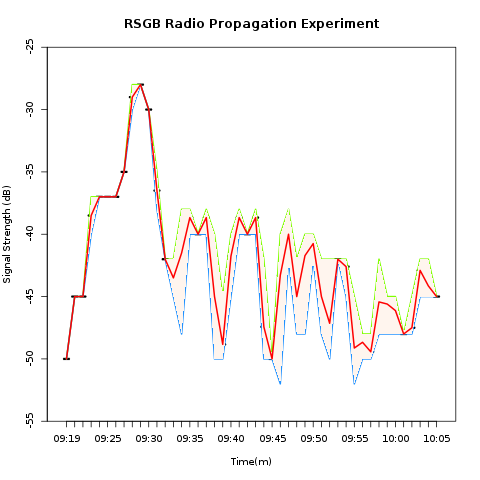
\includegraphics[width=7cm]{images/67}
		\caption{Plot of signal power vs time}
		\label{fig:signal_power_v_time_radio_propagation}
	\end{subfigure}
	\quad
	\begin{subfigure}[t]{7cm}
		\centering
		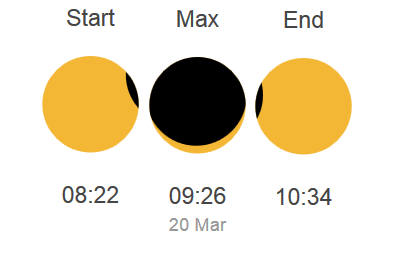
\includegraphics[width=7cm]{images/88}
		\caption{Solar eclipse totality progress}
		\label{fig:solar_eclipse_totality_plot}
	\end{subfigure}
	\caption{20th March 2015 solar eclipse}
	\label{fig:solar_eclipse_20_march_2015}
\end{figure}
%


\newpage
\section*{Capturing DAM Emissions}
\addcontentsline{toc}{section}{Capturing DAM Emissions}
Using the Radio Jupiter Pro software, a prediction was made that 23rd April 2015 would offer a very good opportunity to hear \gls{DAM} emissions. As can be seen in Figure: \ref{fig:dam_emissions_io_a_april_23_prediction}, at the point of the highest chance of capturing \gls{DAM} emissions, Jupiter was right on the very edge of the antenna beam focus. Due to the limitations in the design of the antenna, this configuration offered the best chance to receive an emission from Jupiter.

Despite this, a number of emissions were recorded as can be seen in in the raw image Figure: \ref{fig:dam_emissions_io_a_april_23}. The emissions appear as faint horizontal lines in this waterfall diagram. This diagram is limited by the small bandwidth of 2 MHz and short period of 2 minutes. Ideally in order to spot these interesting emissions a large bandwidth of 20 MHz for instance should be used, over a long period of observation such as 1-24 hours. An example of this is section of a spectrogram seen in Figure: \ref{fig:wide_radio_spectrogram}, which shows averaged signal power data for frequencies 17-55 MHz and 70-1000 MHz for a 24 hour period.


There are many open source software tools such as rtl\_power, simple\_ra and heatmap which could capture averaged raw signal strength data from a RTL based receiver in order to build spectrogram diagrams. Unfortunately most of this software is not compatible with the HackRF. However the basic functionality from these tools can be replicated using basic processing blocks within GNURadio and the spectrograms can be built using tools like Octave or Mathlab.

%
\begin{figure}	
	\centering
	\begin{subfigure}[t]{8cm}
		\centering
		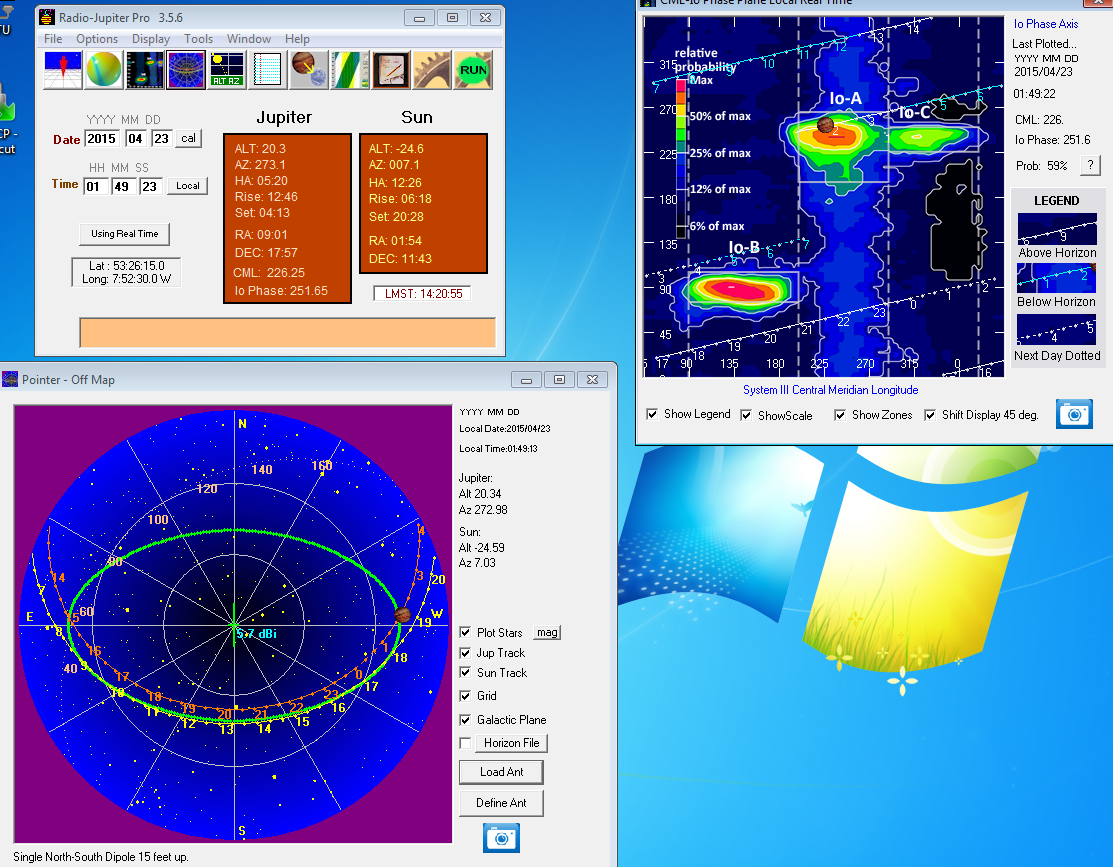
\includegraphics[width=8cm]{images/52}
		\caption{Jupiter \gls{DAM} IO-A Storm Prediction}\label{fig:dam_emissions_io_a_april_23_prediction}		
	\end{subfigure}
	\quad
	\begin{subfigure}[t]{5cm}
		\centering
		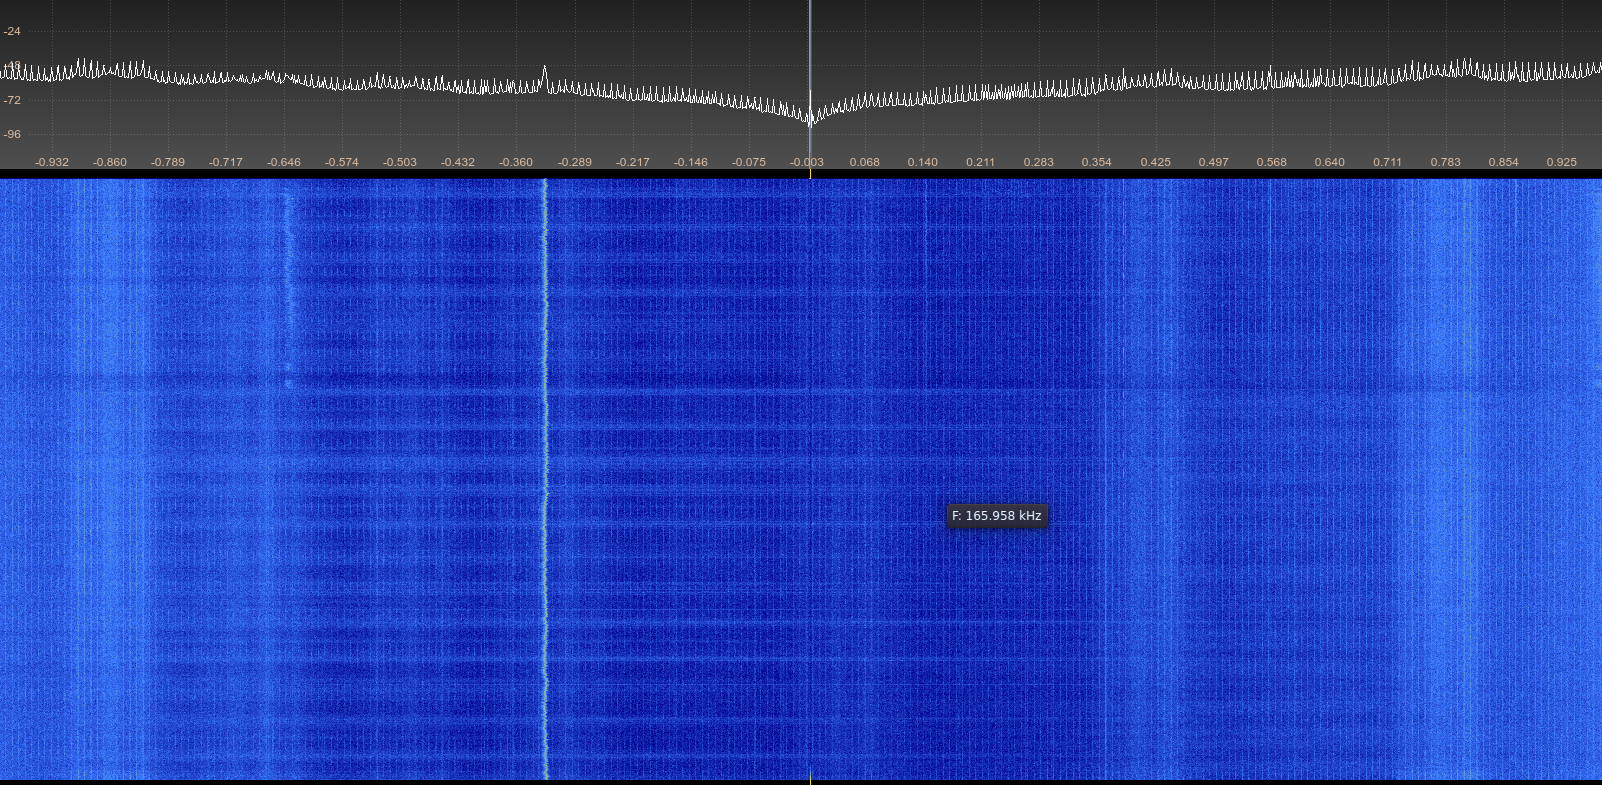
\includegraphics[width=5cm]{images/54}
		\caption{\gls{DAM} emissions picked up during an IO-A storm}
		\label{fig:dam_emissions_io_a_april_23}
	\end{subfigure}
	\quad
	\begin{subfigure}[t]{5cm}
		\centering
		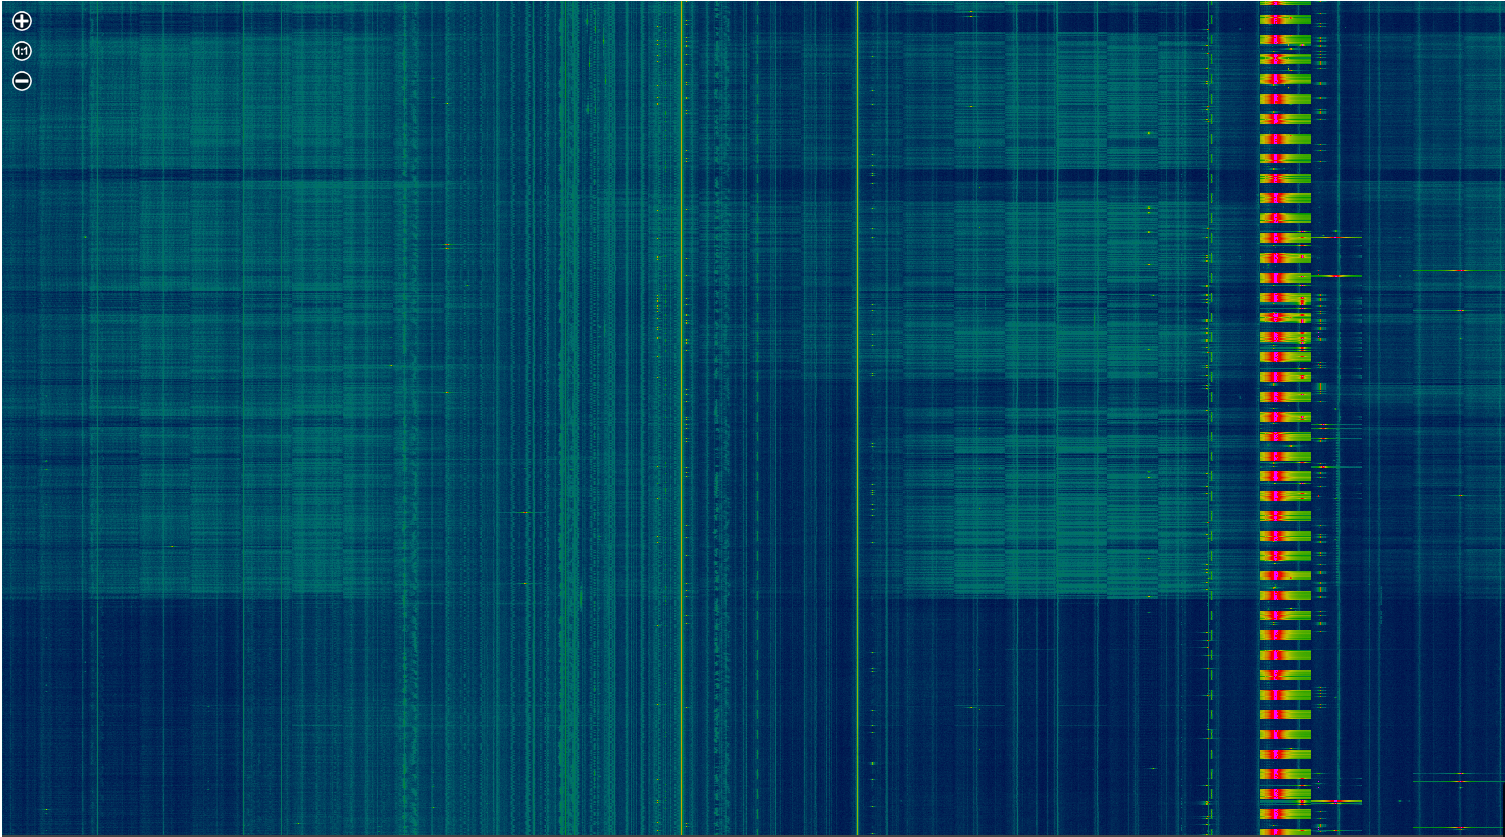
\includegraphics[width=5cm]{images/55}
		\caption{Radio Spectrogram Diagram \citep{superkuh-15}}
		\label{fig:wide_radio_spectrogram}
	\end{subfigure}
	\caption{DAM Emissions}
	\label{fig:jupiter_dam_emissions}
\end{figure}
%